\documentclass[8pt]{article}

\usepackage[T1]{fontenc}
\usepackage[utf8]{inputenc}

\usepackage{pdfpages}
\usepackage{graphicx}
\usepackage{lmodern}
\usepackage{amsmath}
\usepackage{amsthm}
\usepackage{amssymb}
\usepackage{listings}
\usepackage{enumerate}
\usepackage{amsfonts}
\usepackage{float}
\usepackage{listings}
\usepackage[left=2cm,right=2cm,top=2cm,bottom=2cm]{geometry}
\lstset{
basicstyle=\selectfont\footnotesize,
columns=fullflexible,
frame=single,
literate=*{-}{-}1{*}{*}1
}
\usepackage{pdfpages}

\PassOptionsToPackage{hyphens}{url}
\usepackage{hyperref}
\usepackage{color} % gestion de différentes couleurs
\definecolor{linkcolor}{rgb}{0,0,0.6} % définition de la couleur des liens pdf
\hypersetup{
colorlinks,
citecolor=black,
filecolor=black,
linkcolor=linkcolor,
urlcolor=linkcolor
}

\begin{document}
	
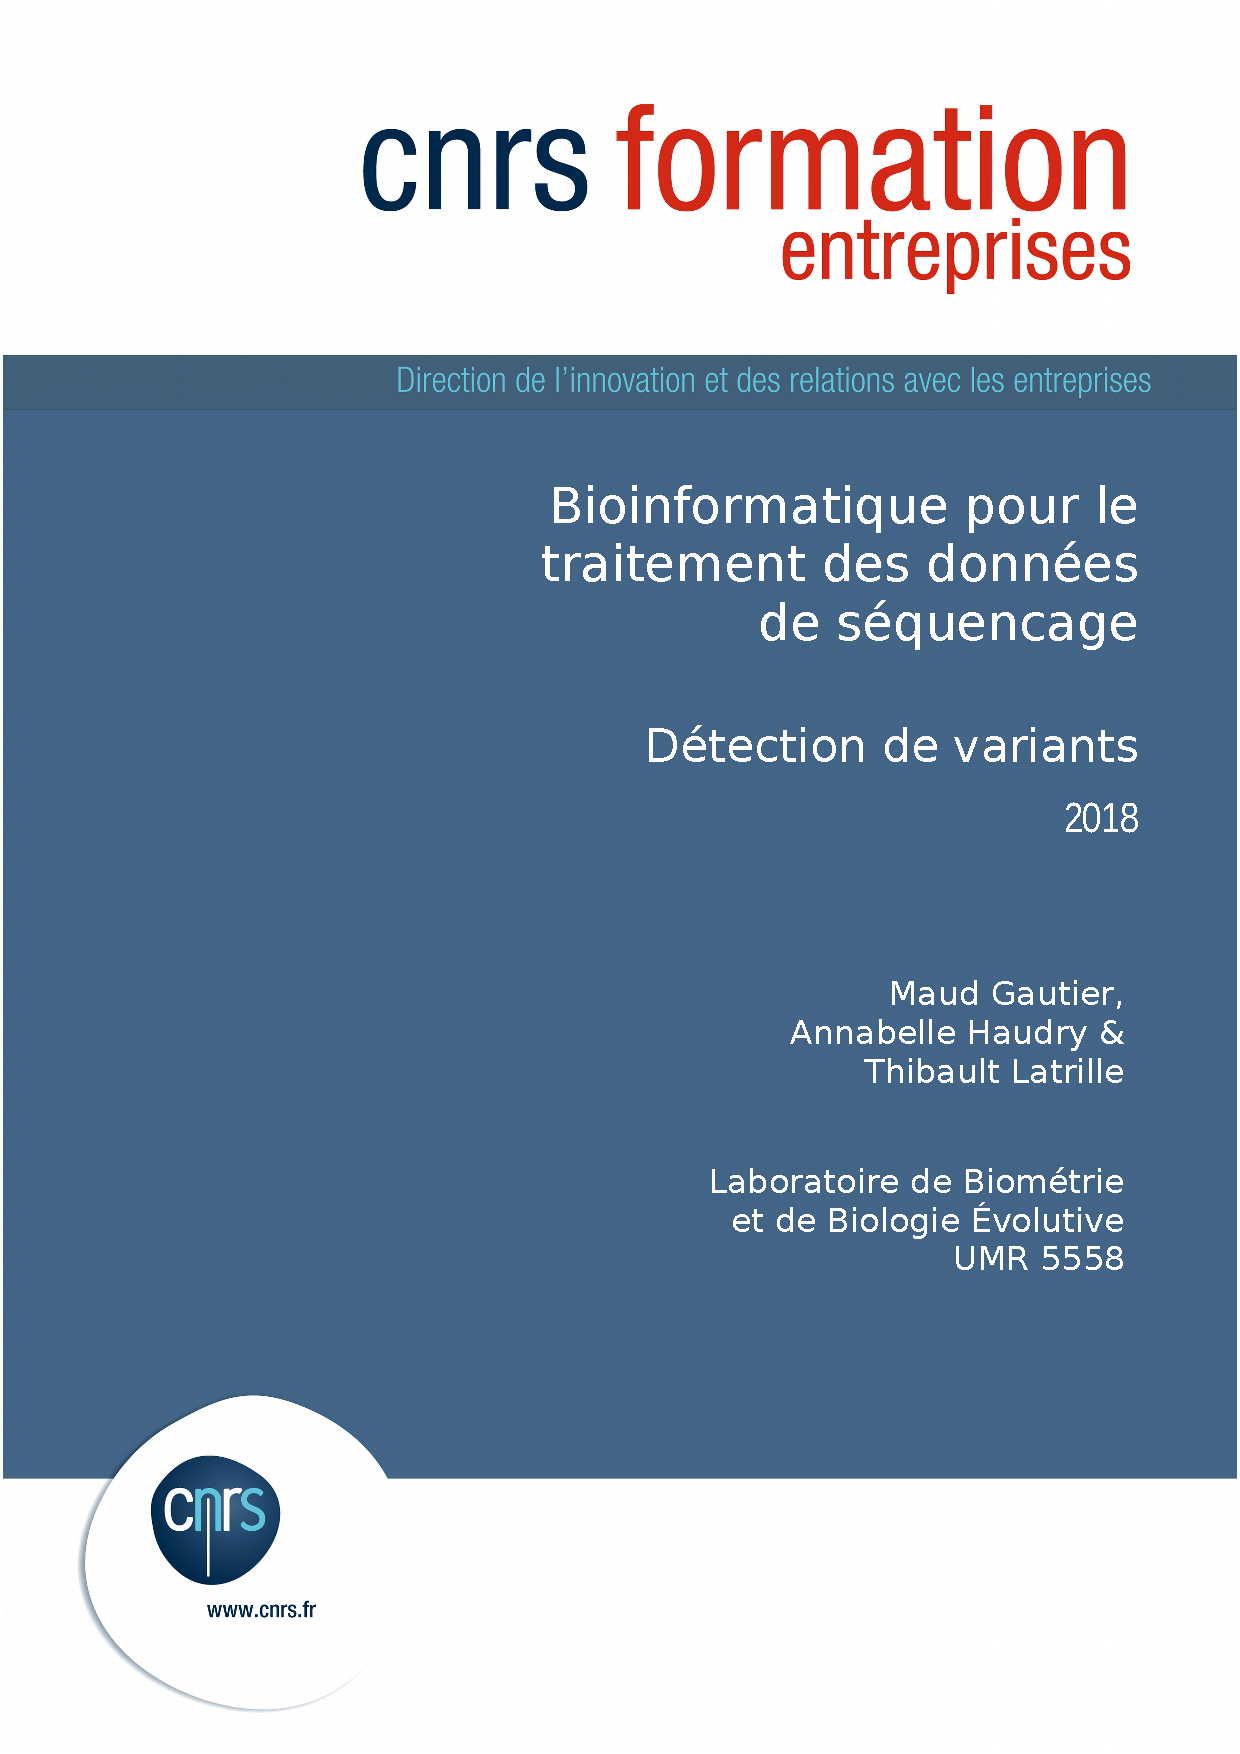
\includepdf[pages={1},scale=1]{couverture.pdf}


\includepdf[pages={2-13},scale=1,nup=1x2]{../presentation/mapping.pdf}

\includepdf[pages={3-22},scale=1,nup=1x2]{../presentation/variant-calling.pdf}


\section*{Data Format}
\subsection*{Fasta}
\textbf{Reference:} \url{https://zhanglab.ccmb.med.umich.edu/FASTA/}\\ 
FASTA format is a text-based format for representing either nucleotide sequences or peptide sequences, in which base pairs or amino acids are represented using single-letter codes. A sequence in FASTA format begins with a single-line description, followed by lines of sequence data. The description line is distinguished from the sequence data by a greater-than (">") symbol in the first column. 
\subsection*{FastQ}
\textbf{Reference:} \url{https://doi.org/10.1093/nar/gkp1137}\\ 
FASTQ format is a text-based format for storing both a biological sequence (usually nucleotide sequence) and its corresponding quality scores. Both the sequence letter and quality score are each encoded with a single ASCII character for brevity. 
\subsection*{SAM/BAM}
\textbf{Reference:} \url{http://samtools.github.io/hts-specs/SAMv1.pdf}\\ 
SAM stands for Sequence Alignment/Map format.  It is a TAB-delimited text format consisting of a header section, which is optional, and an alignment section.  If present, the header must be prior to the alignments. Header lines start with ‘@’, while alignment lines do not.  Each alignment line has 11 mandatory fields for essential alignment information such as mapping position, and variable number of optional fields for flexible or aligner specific information. BAM is the equivalent of a SAM in a binary format, used for compressing the data.
\subsection*{VCF}
\textbf{Reference}: \url{http://samtools.github.io/hts-specs/VCFv4.3.pdf}\\
VCF is a text file format (most likely stored in a compressed manner).  It contains meta-information lines (prefixed with ‘\#\#’), a header line (prefixed with ‘\#’), and data lines each containing information about a position in the genome and genotype information on samples for each position (text fields separated by tabs).  Zero length fields are not allowed, a dot (‘.’) must be used instead.

\section*{Tools}

\subsection*{FastQC}
\textbf{Reference:} \url{http://www.bioinformatics.babraham.ac.uk/projects/fastqc/}\\
FastQC aims to provide a simple way to do some quality control checks on raw sequence data coming from high throughput sequencing pipelines. It provides a modular set of analyses which you can use to give a quick impression of whether your data has any problems of which you should be aware before doing any further analysis. \\
\textbf{Example usage:}
\begin{lstlisting}[language=bash]
$ fastqc ${seq-input-1} ... ${seq-input-n} -t ${nbr-threads} -o ${dir-output}
\end{lstlisting}

\subsection*{IGV}
\textbf{Reference:} \url{http://software.broadinstitute.org/software/igv/book/export/html/6}\\
The Integrative Genomics Viewer (IGV) is a high-performance visualization tool for interactive exploration of large, integrated genomic datasets. It supports a wide variety of data types, including array-based and next-generation sequence data, and genomic annotations.\\
\textbf{Example usage:}
\begin{lstlisting}[language=bash]
$ igv
\end{lstlisting}

\subsection*{Burrows-Wheeler Aligner (BWA)}
\textbf{Reference:} \url{http://bio-bwa.sourceforge.net/bwa.shtml}\\
BWA is a software package for mapping low-divergent sequences against a large reference genome, such as the human genome. It consists of three algorithms: BWA-backtrack, BWA-SW and BWA-MEM. The first algorithm is designed for Illumina sequence reads up to 100bp, while the rest two for longer sequences ranged from 70bp to 1Mbp. BWA-MEM and BWA-SW share similar features such as long-read support and split alignment, but BWA-MEM, which is the latest, is generally recommended for high-quality queries as it is faster and more accurate. BWA-MEM also has better performance than BWA-backtrack for 70-100bp Illumina reads. 
\\
\textbf{Example usage:}
\begin{lstlisting}[language=bash]
$ bwa mem -t ${nbr-threads} -M ${ref-file}.fa ${reads-file}.fq > ${aln-se-file}.sam 
\end{lstlisting}

\subsection*{Samtools}
\textbf{Reference:} \url{http://www.htslib.org/doc/samtools.html}\\
Samtools is a suite of programs for interacting with high-throughput sequencing data. It consists of three separate repositories:
\begin{itemize}
	\item \textbf{Samtools}: Reading/writing/editing/indexing/viewing SAM/BAM/CRAM format
	\item \textbf{BCFtools}: Reading/writing BCF2/VCF/gVCF files and calling/filtering/summarising SNP and short indel sequence variants
	\item \textbf{HTSlib}: A C library for reading/writing high-throughput sequencing data
\end{itemize}
\textbf{Example usage:}
\begin{lstlisting}[language=bash]
$ samtools view -@ ${nbr-threads} ${aln-se-input}.sam -Sbh -f 3 -o ${aln-se-output}.bam
$ samtools sort -@ ${nbr-threads} ${aln-se-input}.bam -o ${aln-se-output}.bam
$ samtools index ${aln-se-input}.bam
$ samtools flagstat ${aln-se-input}.bam > ${stats-output}.txt
$ samtools stats ${aln-se-input}.bam > ${stats-output}.txt
$ samtools merge ${aln-se-output}.bam ${aln-se-input-list}.bamlist
\end{lstlisting}
\subsection*{Picard}
\textbf{Reference:} \url{https://broadinstitute.github.io/picard/command-line-overview.html#Overview}\\
Picard is a set of command line tools for manipulating high-throughput sequencing (HTS) data and formats such as SAM/BAM/CRAM and VCF.\\
\textbf{Example usage:} AddOrReplaceReadGroups replaces read groups in a BAM file. This tool enables the user to replace all read groups in the INPUT file with a single new read group and assign all reads to this read group in the OUTPUT BAM file.
\begin{lstlisting}[language=bash]
$ java -jar ${picard-path} AddOrReplaceReadGroups \
$					INPUT=${aln-se-input}.bam \
$					OUTPUT=${aln-se-output}.bam \
$					RGID=${read-group-identifier}\
$					RGLB=${dna-preparation-library-identifier} \
$					RGPL=${technology-used-to-produce-the-read} \
$					RGPU=${platform-unit} \
$					RGSM=${sample}
\end{lstlisting}
For meaning of the read group see \url{https://software.broadinstitute.org/gatk/documentation/article.php?id=6472}\\
\textbf{Example usage:} MarkDuplicates locates and tags duplicate reads in a BAM or SAM file, where duplicate reads are defined as originating from a single fragment of DNA. 
\begin{lstlisting}[language=bash]
$ java -jar ${picard-path} MarkDuplicates \
$					I=${aln-se-input}.bam \
$					O=${aln-se-output}.bam \
$					METRICS_FILE=${markDup-metrics}.txt
\end{lstlisting}

\subsection*{Genome Analysis Toolkit (GATK)}
\textbf{Reference:} \url{https://software.broadinstitute.org/gatk/documentation}\\
GATK is the industry standard for identifying SNPs and indels in germline DNA and RNAseq data. Its scope is now expanding to include somatic variant calling tools, and to tackle copy number (CNV) and structural variation (SV). In addition to the variant callers themselves, GATK also includes many utilities to perform related tasks such as processing and quality control of high-throughput sequencing data.

These tools were primarily designed to process exomes and whole genomes generated with Illumina sequencing technology, but they can be adapted to handle a variety of other technologies and experimental designs. And although it was originally developed for human genetics, GATK has since evolved to handle genome data from any organism, with any level of ploidy.\\
\textbf{Example usage:} RealignerTargetCreator defines intervals to target for local realignment.
\begin{lstlisting}[language=bash]
$ java -jar ${gatk-path} -T RealignerTargetCreator \
$					-R ${ref-input}.fa \
$					-I ${aln-se-input}.bam \
$					-o ${intervals-output}.txt \
$					--known ./${known-indels-input}.vcf.gz
\end{lstlisting}
\textbf{Example usage :} IndelRealigner performs local realignment of reads around indels
\begin{lstlisting}[language=bash]
$ java -jar ${gatk-path} -T IndelRealigner \
$					-R ${ref-input}.fa \
$					-I ${aln-se-input}.bam \
$					-o ${aln-se-output}.bam \
$					--targetIntervals ${intervals-input}.txt \
$					-known ${known-indels-input}.vcf.gz
\end{lstlisting}
\textbf{Example usage :} BaseRecalibrator generates base recalibration table to compensate for systematic errors in basecalling confidences.
\begin{lstlisting}[language=bash]
$ java -jar ${gatk-path} -T BaseRecalibrator -l INFO \
$					-R ${ref-input}.fa \
$					-I ${aln-se-input}.bam \
$					-o ${cov-table-output}.table \
$					-cov ReadGroupCovariate \
$					-cov QualityScoreCovariate \
$					-cov CycleCovariate -cov ContextCovariate \
$					-knownSites ${known-snps-input}.vcf.gz
\end{lstlisting}
\textbf{Example usage :} PrintReads is a generic utility tool for manipulating sequencing data in SAM/BAM format. When PrintReads is used as part of the Base Quality Score Recalibration workflow, it takes the `--BQSR` engine argument.
\begin{lstlisting}[language=bash]
$ java -jar ${gatk-path} -T PrintReads \
$					-R ${ref-input}.fa \
$					-I ${aln-se-input}.bam \
$					-o ${aln-se-output}.bam \
$					-BQSR ${cov-table-input}.table
\end{lstlisting}
\textbf{Example usage:} HaplotypeCaller calls germline SNPs and indels via local re-assembly of haplotypes.
\begin{lstlisting}[language=bash]
$ java -jar ${gatk-path} -T HaplotypeCaller \
$					-R ${ref-input}.fa \
$					-I ${aln-se-input}.bam \
$					-o ${var-call-output}.gvcf \
$					--genotyping_mode DISCOVERY \
$					-variant_index_type LINEAR \
$					-variant_index_parameter 128000 \
$					--emitRefConfidence GVCF
\end{lstlisting}
\textbf{Example usage:} GenotypeGVCFs performs joint genotyping on gVCF files produced by HaplotypeCaller.
\begin{lstlisting}[language=bash]
$ java -jar ${gatk-path} -T GenotypeGVCFs \
$					-R ${ref-input}.fa \
$					--variant ${var-call-input-1}.gvcf \
$					...
$					--variant ${var-call-input-n}.gvcf \
$					-o ${var-call-output}.vcf
\end{lstlisting}

\newpage

\textbf{Example usage:} PhaseByTransmission computes the most likely genotype combination and phasing for trios and parent/child pairs.
\begin{lstlisting}[language=bash]
$ java -jar ${gatk-path} -T PhaseByTransmission \
$					-R ${ref-input}.fa \
$					-V ${var-call-input}.vcf \
$					-ped ${pedigree-input}.ped \
$					-o ${var-call-output}.vcf
\end{lstlisting}
\textbf{Example usage:} GenotypeConcordance takes in two callsets (vcfs) and tabulates the number of sites which overlap and share alleles.
\begin{lstlisting}[language=bash]
$ java -jar ${gatk-path} -T GenotypeConcordance \
$					-R ${ref-input}.fa \
$					-eval ${var-call-input-1}.vcf \
$					-comp ${var-call-input-2}.vcf \
$					-o ${genotype-concordance-output}.txt
\end{lstlisting}
\textbf{Example usage:} VariantEval calculates various quality control metrics, such as the number of raw or filtered SNP counts; ratio of transition mutations to transversions; concordance of a particular sample's calls to a genotyping chip; number of singletons per sample; etc
\begin{lstlisting}[language=bash]
$ java -jar ${gatk-path} -T VariantEval \
$					-R ${ref-input}.fa \
$					-eval:set1 ${var-call-input-1}.vcf \
$					...
$					-eval:setn ${var-call-input-n}.vcf \
$					-o ${variant-eval-output}.txt
\end{lstlisting}

\end{document}